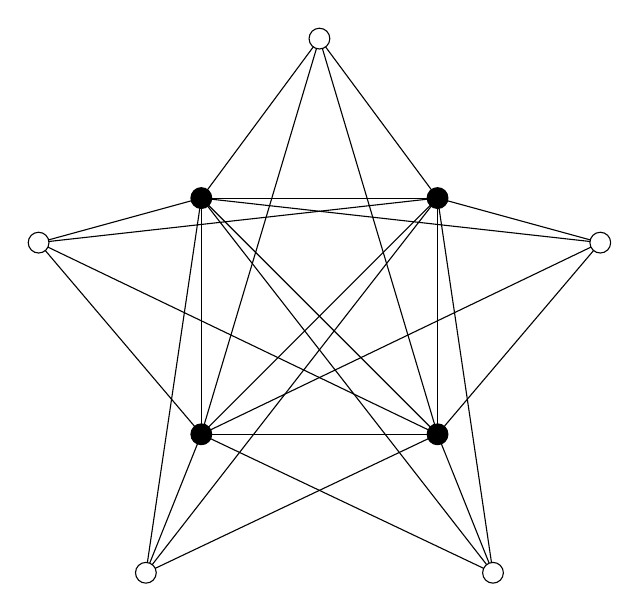
\begin{tikzpicture}[scale=0.75]
\coordinate (a1) at (0,5);
\coordinate (a2) at ({5*sin(72)},{5*cos(72)});
\coordinate (a3) at ({5*sin(144)},{5*cos(144)});
\coordinate (a4) at ({5*sin(216)},{5*cos(216)});
\coordinate (a5) at ({5*sin(288)},{5*cos(288)});
\coordinate (b1) at (2,2.3);
\coordinate (b2) at (-2,2.3);
\coordinate (b3) at (-2,-1.7);
\coordinate (b4) at (2,-1.7);
\draw (a1) -- (b1);
\draw (a1) -- (b2);
\draw (a1) -- (b3);
\draw (a1) -- (b4);
\draw (a2) -- (b1);
\draw (a2) -- (b2);
\draw (a2) -- (b3);
\draw (a2) -- (b4);
\draw (a3) -- (b1);
\draw (a3) -- (b2);
\draw (a3) -- (b3);
\draw (a3) -- (b4);
\draw (a4) -- (b1);
\draw (a4) -- (b2);
\draw (a4) -- (b3);
\draw (a4) -- (b4);
\draw (a5) -- (b1);
\draw (a5) -- (b2);
\draw (a5) -- (b3);
\draw (a5) -- (b4);
\draw (b1) -- (b2);
\draw (b1) -- (b3);
\draw (b1) -- (b4);
\draw (b2) -- (b3);
\draw (b2) -- (b4);
\draw (b3) -- (b4);
\draw[fill=white] (a1) circle (5pt);
\draw[fill=white] (a2) circle (5pt);
\draw[fill=white] (a3) circle (5pt);
\draw[fill=white] (a4) circle (5pt);
\draw[fill=white] (a5) circle (5pt);
\draw[fill=black] (b1) circle (5pt);
\draw[fill=black] (b2) circle (5pt);
\draw[fill=black] (b3) circle (5pt);
\draw[fill=black] (b4) circle (5pt);
\end{tikzpicture}